\providecommand{\topdir}{..}
\documentclass[../main.tex]{subfiles}

%External sources
\graphicspath{{\topdir/img/02/}}

\begin{document}

\section{Historical evolution of vision mixers}
The first vision mixers were introduced into the market as soon as the first commercial \gls{tv} broadcasters began operations in the early 1940s\cite{ArmesRoy1988Ov}. At that time, vision mixers operated in a mechanical manner, this is, they merely consisted of switch matrices used to route input signals to the main output. As no signal processing was performed, all inputs needed to be \textit{genlocked}; In other words, their horizontal sync pulses needed to happen at the same time\cite{becg2020}.\newline

As time passed, these commutation matrices evolved into complex mixers, which allowed to perform several effects using analog electronics, although they still needed \textit{genlocked} sources. For instance, these mixers were able to fade or wipe between sources, or compose using \textit{luma key}s\cite{WardPeter2001Saob}. This same time, the standard program-preset operation model was introduced, as opposed to the older A-B model. The mixer displayed in the figure \ref{fig:piher} features both an A-B and a program-preview bank.\newline

\begin{figure}[hbtp]
    \centering
    \subfigure{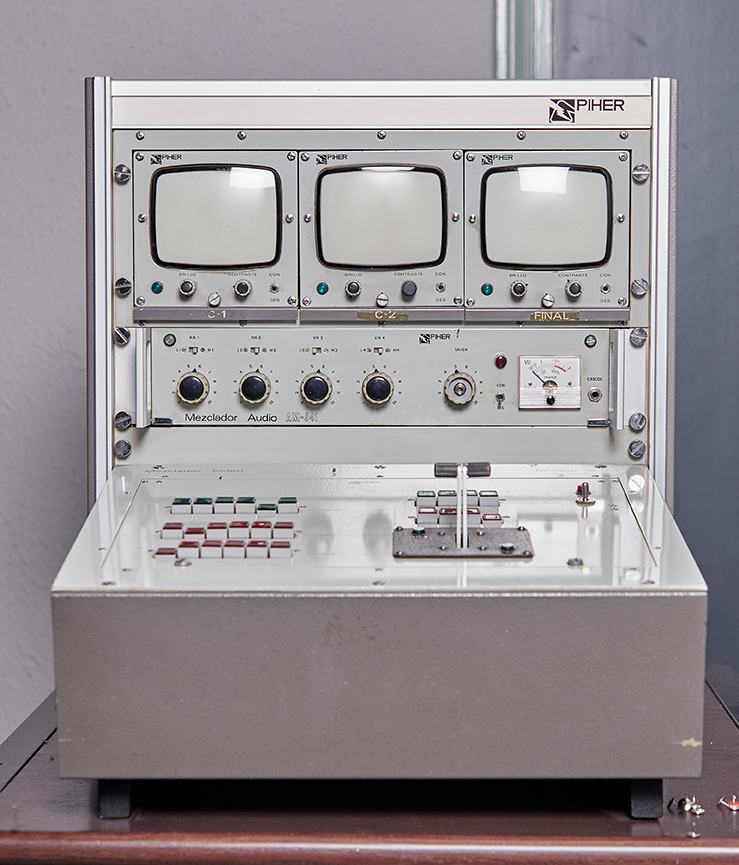
\includegraphics[height=6.5cm]{piher1}}
    \subfigure{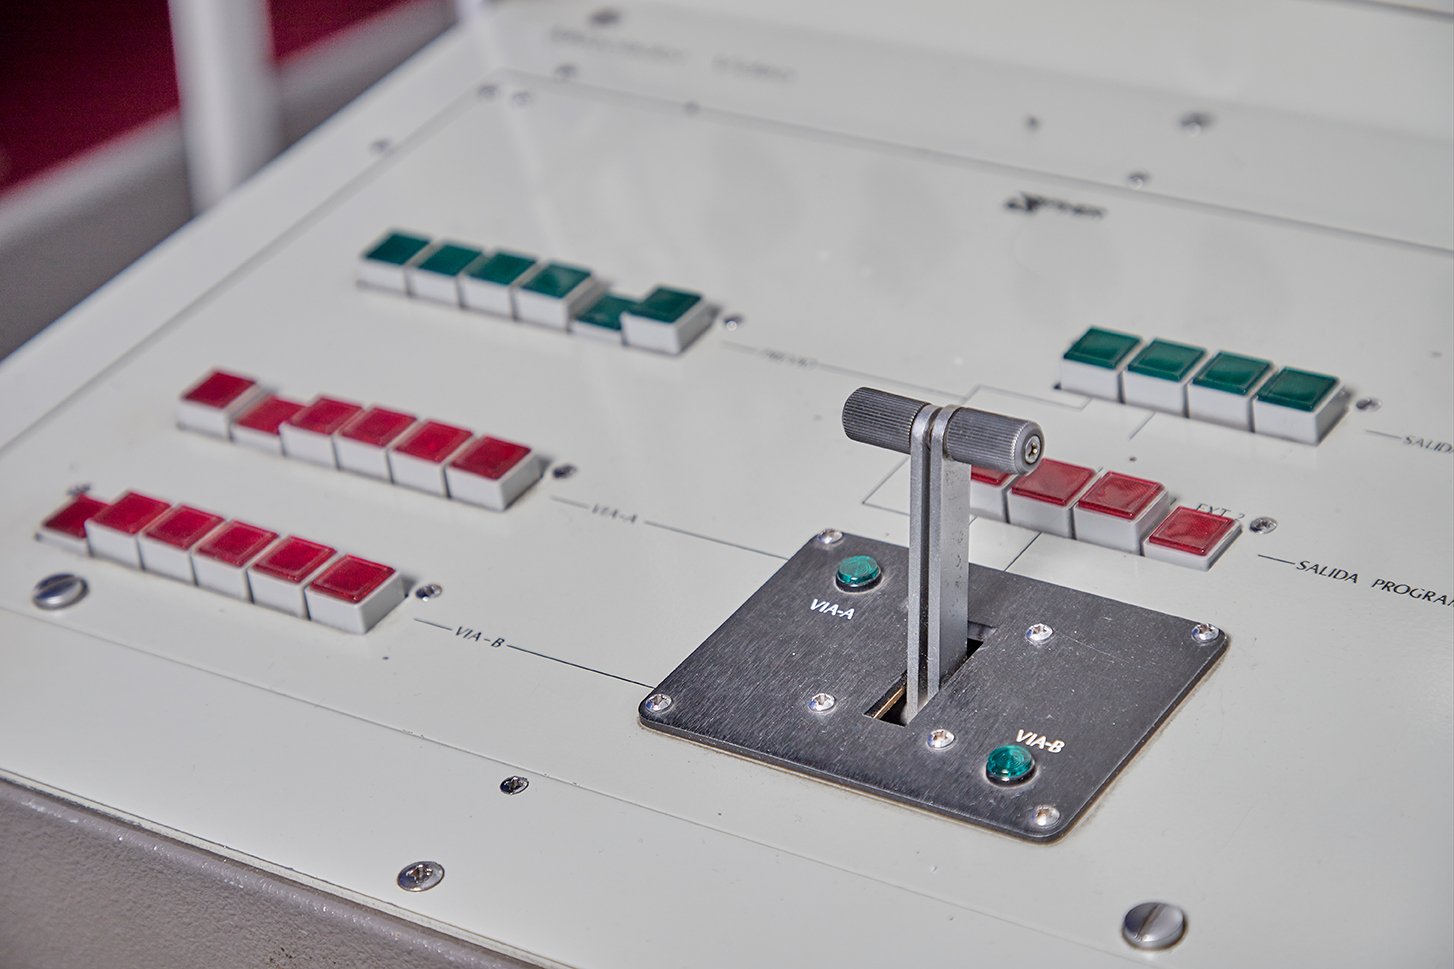
\includegraphics[height=6.5cm]{piher2}}
    \footnotesize{Photos by Facultad de Ciencias de la Información, Universidad Complutense de Madrid}

    \caption{Piher vision mixer, circa 1960}
    \label{fig:piher}
\end{figure}

Shortly after, in the late 1960s some \gls{tv} stations began broadcasting colour signals. This implies that vision mixer technology needed to evolve to handle these new signals. The presence of colour was useful to introduce a powerful technique which is still used: \textit{chroma keying}\cite{jpeters}\cite{tmMixerHistory}. This gives the ability to delete parts of a frame based on its colour. It is typically used in weather forecasts; the presenter sits in front of a green screen which gets swapped with a weather map by the vision mixer.\newline

Several years later, advancements in digital \gls{ic} manufacturing made possible to manipulate video digitally\cite{kitplus2015}. This introduced discrete digital effect processors, known as \glspl{dve}. These allowed spatial transformations of video frames, which were impractical with analog electronics, as high bandwidth signal delays would be needed. Shortly after, these discrete effect processors were integrated into the mixers. Nowadays, although the whole pipeline of the mixers is digital, the \gls{dve} term is still used to refer to those effects which involve spatial transformations of a frame\cite{OwensJim2020Tp}\cite{UtterbackAndrew2015STPa}.\newline

There was a short period in the late 1980s where all video processing was performed with digital electronics but the video \gls{io} was performed using analog signals by the means of \glspl{adc} and \glspl{dac}. This suddenly changed with the introduction of the \gls{sdi} communications protocol, which allows transmitting video alongside ancillary data over a $75 \si{\ohm}$ coaxial cable\cite{ortizrodriguez2018}. This protocol is still used on its latest revision, which allows sending a stream of $12 \si{\giga b \per\second}$. Moreover, it has been adapted to support other transmission mediums such as optical fiber.\newline

The latest advancements came in the late 2000s with the introduction of the first software-based mixers by NewTek. At this same time, the first \gls{ip} based production protocols were introduced. In short terms, \gls{ip} based production replaces the dedicated coaxial cables with the more versatile Ethernet cables. These in turn can be twisted-pair shielded cables or optical fiber. \Gls{ip} based production and software-based mixers work well together, as they facilitate live video production with no dedicated broadcasting equipment.\newline


\section{Common vision mixer features}
Modern vision mixers usually integrate many simpler mixers, known as \gls{me} banks. Each of these units is a full-fledged mixer, which will be responsible of generating a single composition. However, they might generate more than one distinct output signal for reasons that will be explained later. In rough terms, the category of a vision mixer can be measured by its amount of \gls{me} units, although this is quite simplistic, as the feature set of each one of these banks may be more important, but more often than not, there is a certain amount of linearity among these two specifications. Most mixers in the market have 1 to 4 \gls{me} units, topping out at 8.\newline

Each \gls{me} has a signal matrix known as the \textit{crosspoint}. It serves as a router for input signals, which are represented as columns. Meanwhile, each of the feeds required by the \gls{me} will be represented as a row, which can only be fed by one or zero input signals.\newline

\Glspl{me} are based on the program/preview operation model. This operation model consists in configuring the next composition in advance at the preview bus. Meanwhile, the program bus is permanently on air. When the time is right, the contents of the preview bus are swapped with the contents of the program bus, either by an instantaneous cut or a transition. This gives the operator the ability to double check for errors in the composition before it is broadcasted. However, manual changes in the program bus can be performed, although it is not a good operation practice, as any composition error will be instantaneously transmitted.\newline

Each of the composition buses are founded on the background layer. This layer is always visible -although it may be black or transparent- and encompasses the whole screen. As suggested by its name, its only ability is to display a video signal in the background. If no compositing is required, it is used to display the main video feed.\newline

A general view of the signal path on a hypothetical 8-input \gls{me} unit can be seen in the figure \ref{fig:me_signal_path}.\newline

\begin{sidewaysfigure}[hbtp]
    \centering
    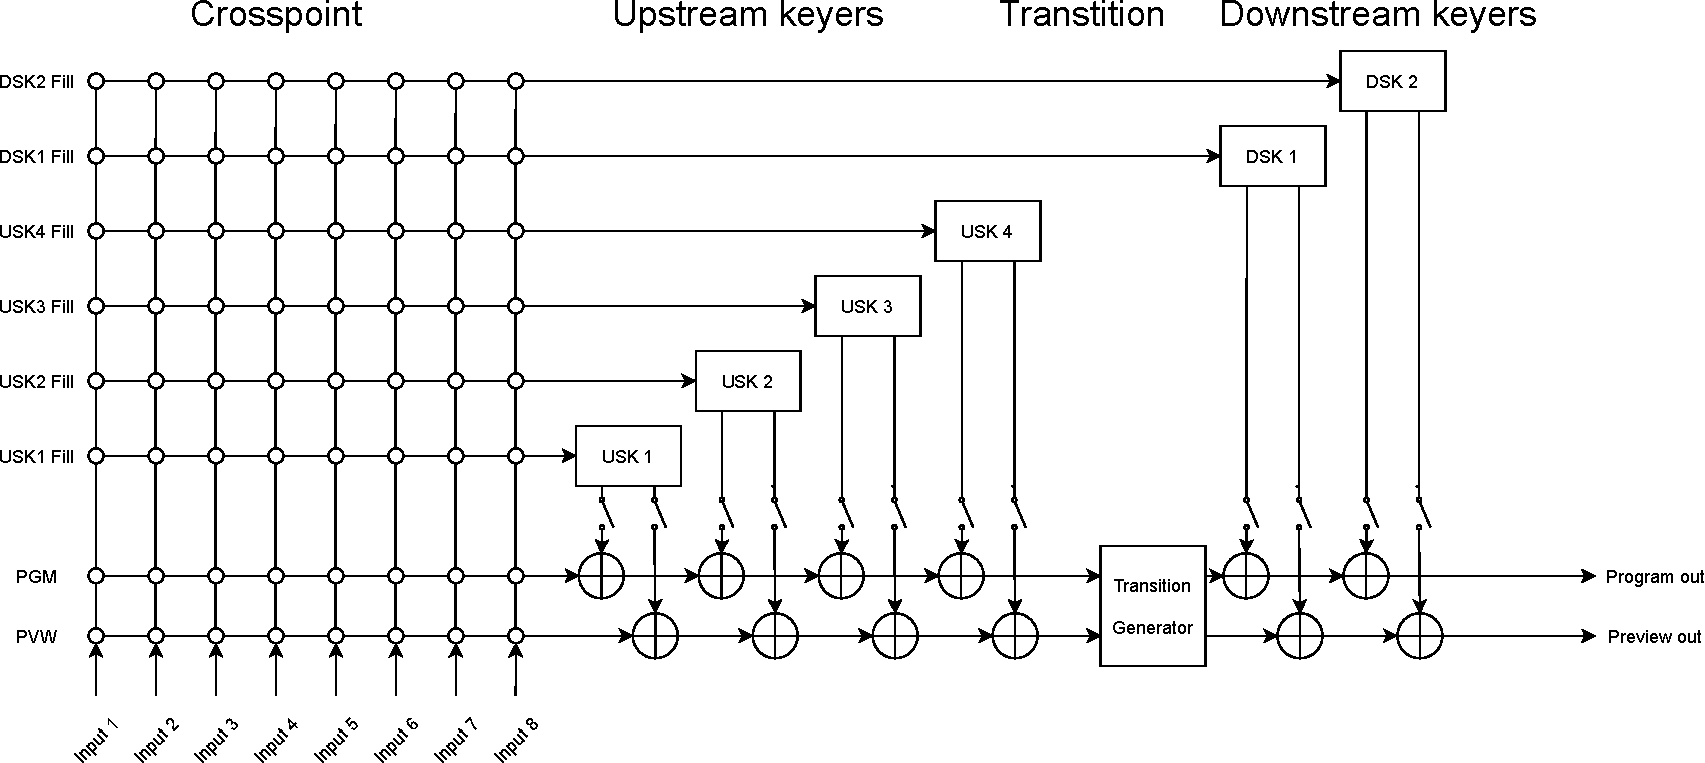
\includegraphics[width=\textwidth]{ME Block Diagram}

    \label{fig:me_signal_path}
    \caption{Signal path on a hypothetical ME with 8 inputs, 4 USKs and 2 DSKs}
\end{sidewaysfigure}

\subsection{Keying}
As mentioned earlier, each of the composition buses has a background layer. Several layers called \textit{keyers} may be added on top of this background. These layers in turn can be classified as \glspl{usk} and \glspl{dsk}. The difference between these two is that \glspl{usk} are added before the transition generator whilst \glspl{dsk} are added to the signal that has the transition already on it. If the transition is inactive, it can be considered that \glspl{dsk} have a higher priority, so they will occlude \glspl{usk}. Usually the \glspl{usk} are used to perform compositions that are background dependant. Meanwhile, the \glspl{dsk} are used to add more stationary contents, such as banners and \gls{tv} station watermarks. Therefore, most vision mixers offer more \glspl{usk} compared to the number of \glspl{dsk}. A possible use case of each one of them is shown in the figure \ref{fig:usk_dsk_example}. \textit{Keyers} can use many different techniques to overlay their image over the background. These techniques will be addressed in their corresponding sections. \newline
 
\begin{figure}[hbtp]
    \centering
    
\includegraphics[width=.8\textwidth]{usk_dsk}

    Note: Both \glspl{usk} are \glspl{dve}. The \gls{dsk} is a linear keyer.
    \caption{Possible use case of USKs and DSKs}
    \label{fig:usk_dsk_example}
\end{figure}


\subsubsection{Linear keying}
This is one of the oldest keying techniques. It consists in using a matte signal which represents the transparency of the filling signal. Sometimes, if a signal carries its own matte information, it is said that it has an alpha channel. The most common usage of the linear key is to overlay \glspl{cg} or other types of computer generated graphics. For instance, the \gls{dsk} shown in the figure \ref{fig:usk_dsk_example} could be using this technique. Unlike other types of keying, it requires two video sources -apart from the background signal- as seen in the figure \ref{fig:linear_key_example}.

\begin{figure}[hbtp]
    \centering
    \subfigure[Fill image]{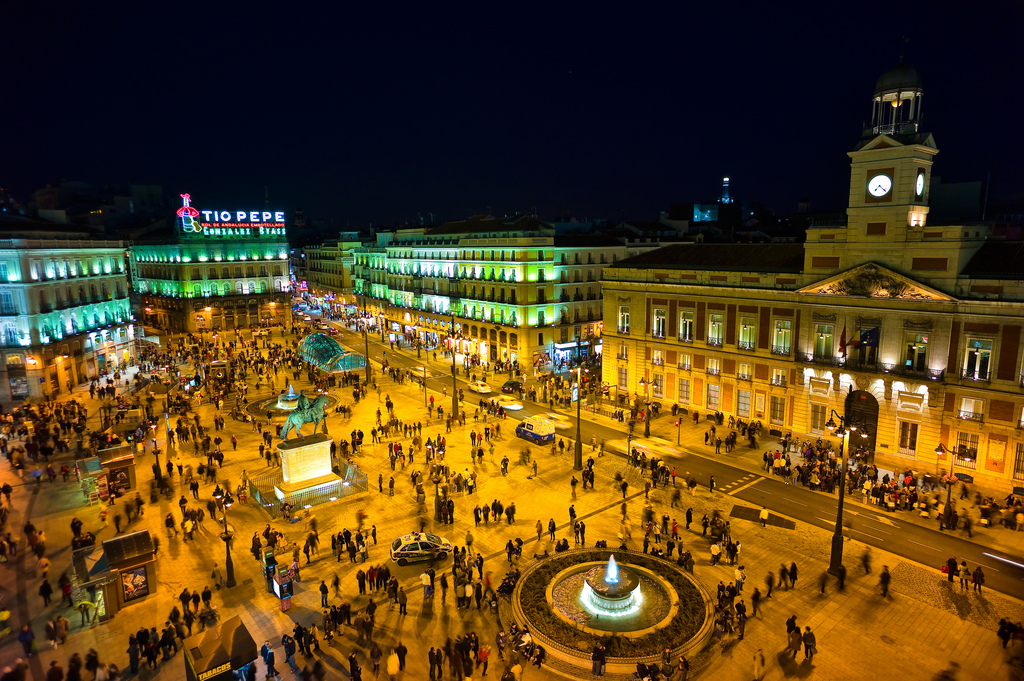
\includegraphics[height=3cm]{linear_fill}}
    \subfigure[Matte image]{
\includegraphics[height=3cm]{linear_key}}
    \subfigure[Linear keyed image]{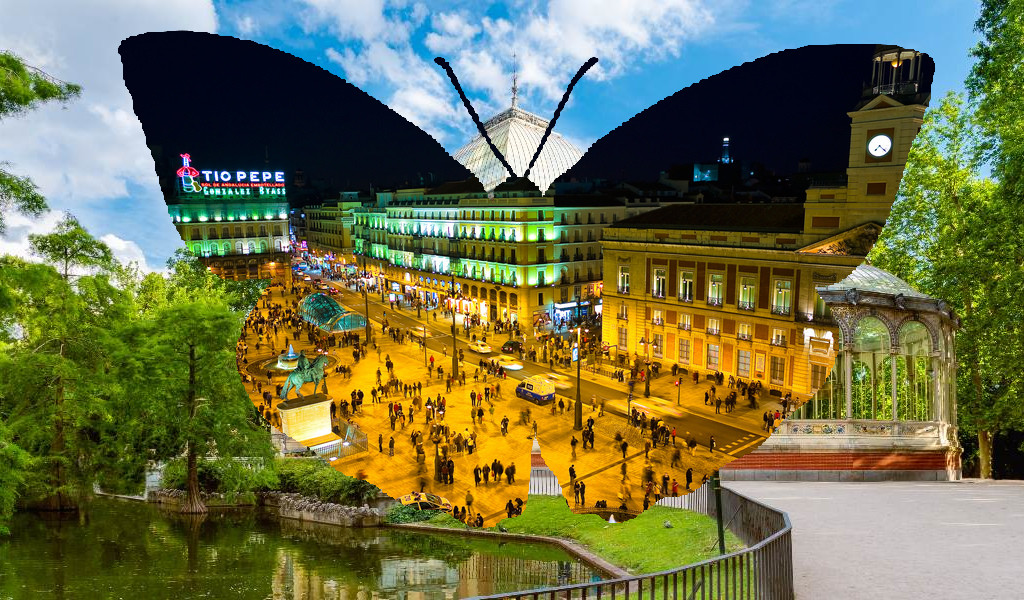
\includegraphics[height=3cm]{linear_comp}}

    \caption{Luma key example}
    \label{fig:linear_key_example}
\end{figure}

\subsubsection{Luma keying}
This type of keying is very similar to the linear key. However, instead of using a dedicated signal for transparency information, it uses its own luminosity. This is only useful if the transparent parts are very black and opaque parts are very white or vice versa. As the luminosity information can not be controlled separately, these keyers usually have more advanced controls, such as lower and upper thresholds, custom transfer functions, and a toggle for inverting the result. An example of this type of keying is displayed in the figure \ref{fig:luma_key_example}.

\begin{figure}[hbtp]
    \centering
    \subfigure[Background image]{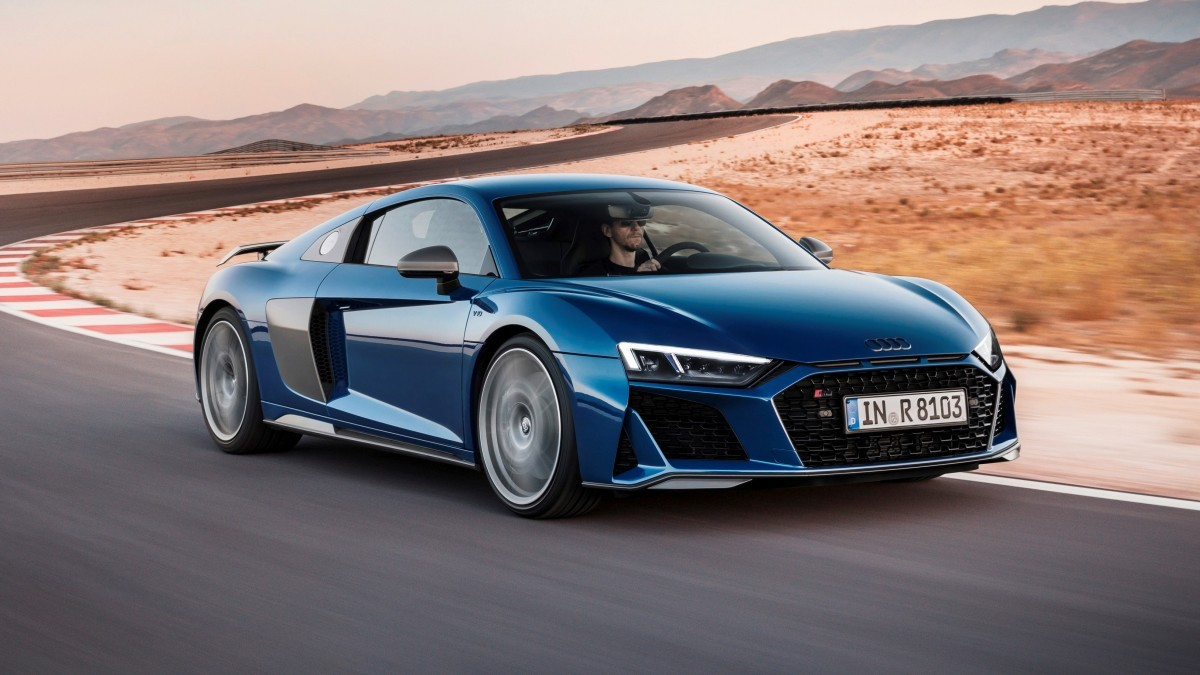
\includegraphics[height=2.8cm]{luma_bkgd}}
    \subfigure[Key source]{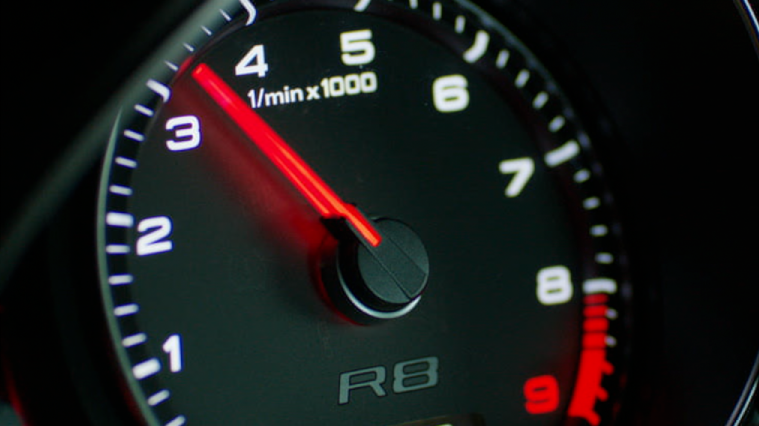
\includegraphics[height=2.8cm]{luma_fill}}
    \subfigure[Luma keyed image]{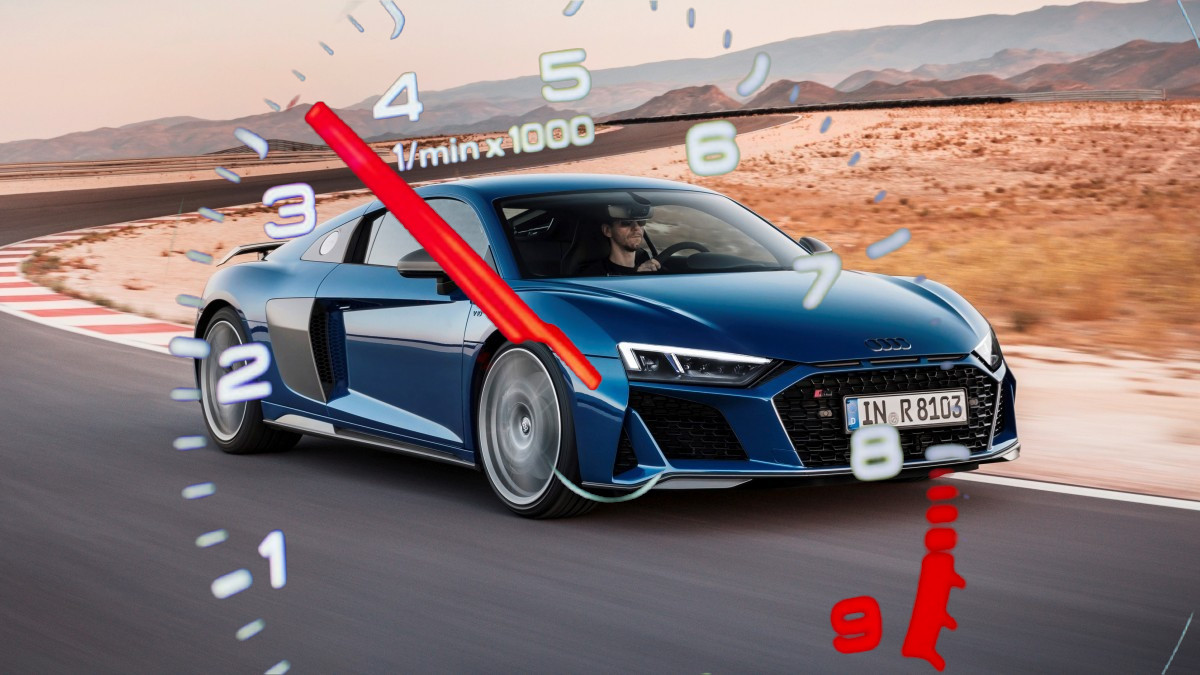
\includegraphics[height=2.8cm]{luma_comp}}

    \caption{Luma key example}
    \label{fig:luma_key_example}
\end{figure}

\subsubsection{Chroma keying}
As opposed to luma keying, chroma keying uses the color information of a video signal to discriminate transparent and opaque parts of an image. This keying is sometimes referred as the \textit{green-screen effect}, as it is usually configured to reject the green color\cite{ortizrodriguez2018}. An example of this effect is shown in the figure \ref{fig:chroma_key_example}.\newline

\begin{figure}[hbtp]
    \centering
    \subfigure[Background image]{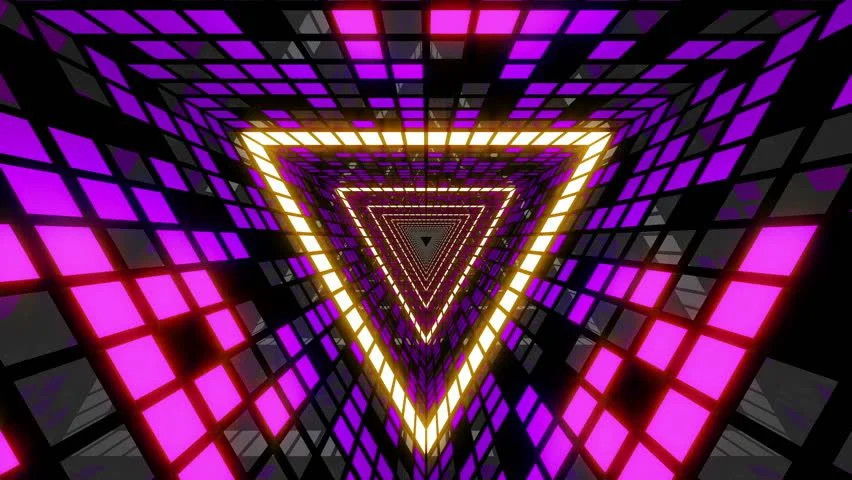
\includegraphics[height=2.8cm]{chroma_bkgd}}
    \subfigure[Key source]{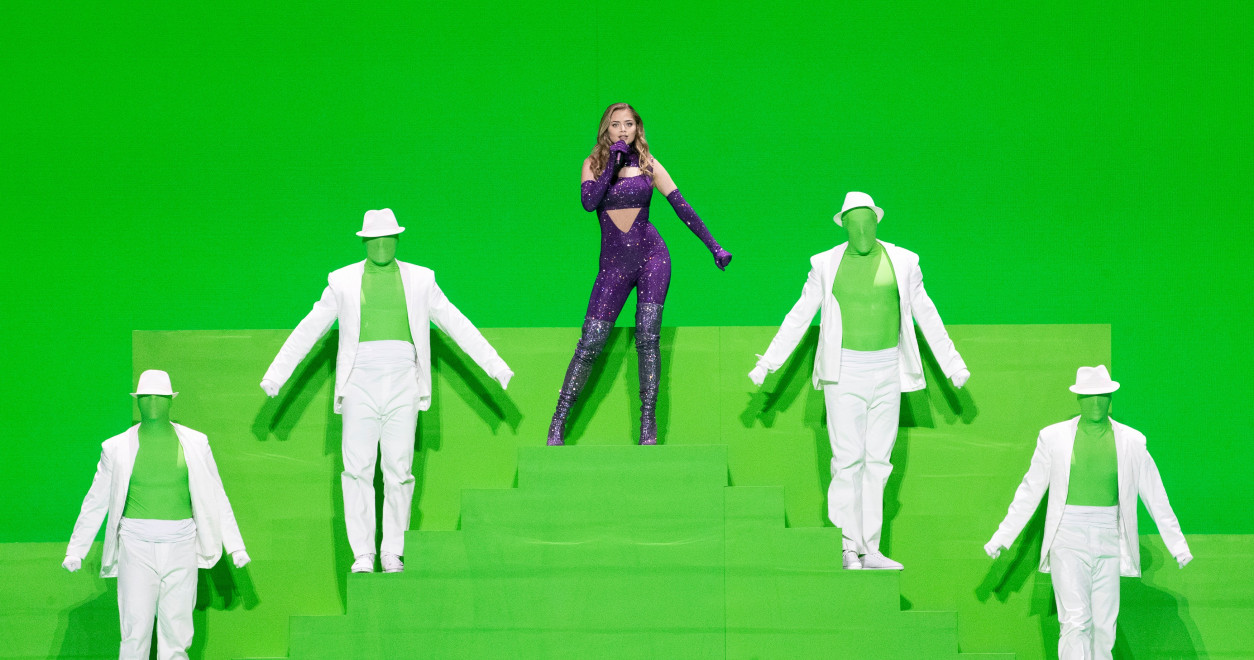
\includegraphics[height=2.8cm]{chroma_fill}}
    \subfigure[Chroma keyed image]{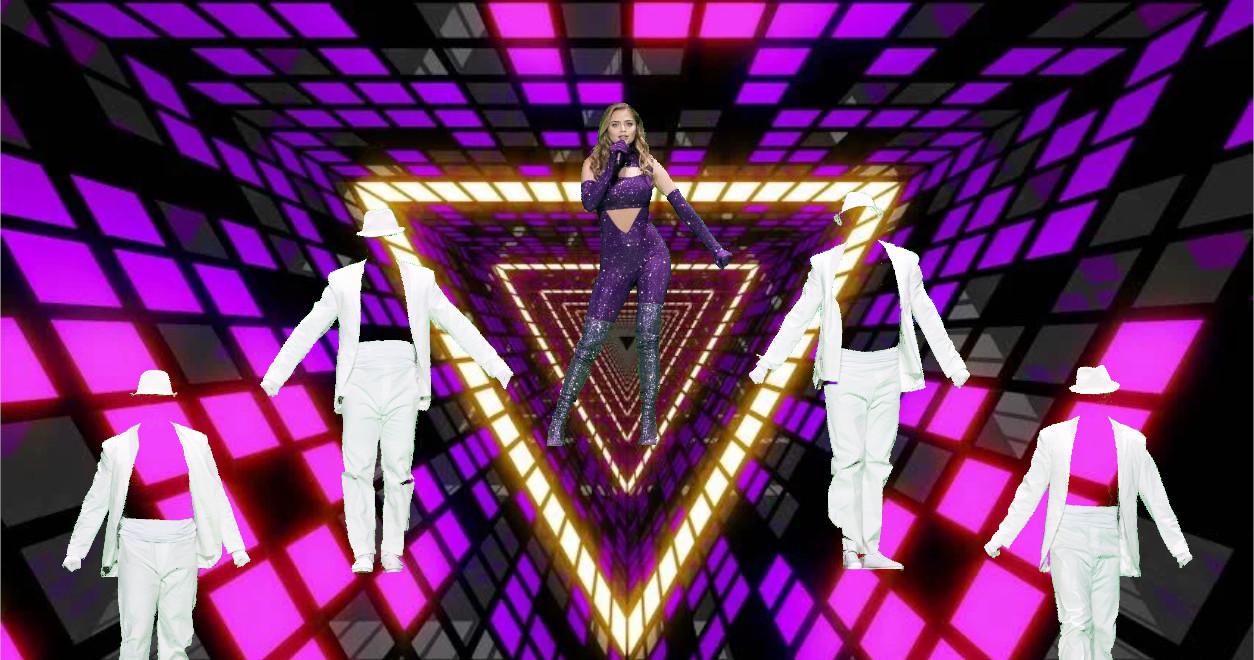
\includegraphics[height=2.8cm]{chroma_comp}}

    \caption{Chroma key example}
    \label{fig:chroma_key_example}
\end{figure}

\subsubsection{DVEs}
The \gls{dve} term refers to the ability to perform geometrical transformations on an overlay. This includes scaling, rotating and positioning an overlay in space. Some mixers offer the ability to perform more complex spatial transformations like 3D effects. It is usually paired with animation controls, as it is useful to give dynamism to these effects.



\subsection{Transitions}
As mentioned earlier, \glspl{me} have two compositing buses which can be swapped with a transition. This transition is applied to the signal that carries the background information with the \glspl{usk} overlaid. Mixers offer several transition effects, the most basic of which will be explained hereunder.

\subsubsection{Mix}

\subsubsection{Wipe}

\subsubsection{DVE-based}




\section{Software based vision mixers}


\section{IP based production}
As mentioned earlier, \gls{ip} based production consists in using standard computer networking infrastructures to transport video inside a \gls{tv} production facility. This video signal is packetized and transmitted using specifically designed protocols and codecs.\newline

As opposed to the traditional streaming, \gls{ip} based production must meet some additional requirements. For instance, the quality of the image must be comparable to the quality provided by uncompressed \gls{sdi}. This rules out using any heavy compression algorithms. Moreover, the latency must be as low as possible, making it impossible to use bidirectional frame compression. Additionally, the signal must fit into a $1 \si{\giga b \per\second}$ or $10 \si{\giga b \per\second}$ link. Finally, it must be able to carry some ancillary data from and to the source.\newline

The first protocol to perform such a task was introduced in 2007 as the SMPTE-2022. This protocol allows sending a MPEG-2 stream or a packetized SD-SDI stream over a $1 \si{\giga b \per \second}$ Ethernet cable\cite{tmIpProduction}. Later in 2017, this standard was upgraded to the SMPTE-2110, which brings many benefits, such as better synchronization mechanisms and support for any resolution, including those larger than \gls{uhd}, as long as there is enough bandwidth \cite{smpte2110faq}. The largest problem with the SMPTE-2110 protocol is that it is not meant to be used by computers, specially in the case of \gls{uhd} signals, as the bitrate is too high for modern \glspl{cpu}.\newline

Another proliferating protocol is NewTek's \gls{ndi}, which is a royalty-free standard. As opposed to SMPTE's \gls{ip} based production protocols, it is paired with a intra-frame compression codec, although it is able to transport existing video codecs such as h264 and h265. This makes it possible to use it with standard networking gear and modest computers whilst keeping resolutions up to \gls{uhd}. Their own codec has been designed to meet the quality requirements mentioned earlier.

\end{document}
